% !TEX program = pdflatex
% !TEX options = -shell-escape -synctex=1 -interaction=nonstopmode -file-line-error "%DOC%"
%\documentclass[multi={mymath},border=2,crop]{standalone}
\documentclass{article}
\usepackage{amsmath}
\usepackage{amssymb}
\usepackage{amsfonts}
\usepackage{tikz}
\usetikzlibrary{intersections,external}
\tikzexternalize[prefix=tikz/]
\usepackage{tikz-cd}

%%% CONVERT: pdf2svg diagrams.pdf figure-%d.svg all

\begin{document}

\tikzsetnextfilename{intersection}

\def\firstcircle{(0,0) circle (1.5cm)}
\def\secondcircle{(2,0) circle (1.5cm)}
\def\thirdcircle{(1,-2) circle (1.5cm)}
\colorlet{circle edge}{black}
\colorlet{circle area}{blue!20}
\tikzset{filled/.style={fill=circle area, draw=circle edge, thick},
	outline/.style={draw=circle edge, thick}}
\setlength{\parskip}{5mm}
\begin{tikzpicture}
\begin{scope}
\clip \firstcircle;
\fill[filled] \secondcircle;
\end{scope}
\draw[outline] \firstcircle node {$A$};
\draw[outline] \secondcircle node {$B$};
\end{tikzpicture}

\tikzsetnextfilename{disjoint}

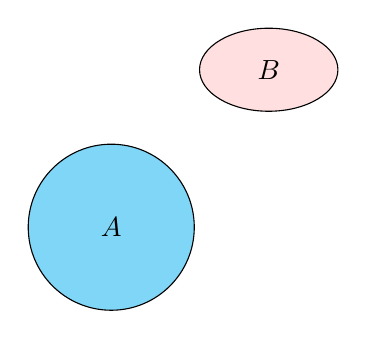
\begin{tikzpicture}
\draw[fill=cyan!50] circle (3em) node {$A$};
\draw[fill=pink!50] (2,2) ellipse  (2.5em and 1.5em) node {$B$};
\end{tikzpicture}
	


\tikzsetnextfilename{union}

\def\firstcircle{(0,0) circle (1.5cm)}
\def\secondcircle{(2,0) circle (1.5cm)}
\def\thirdcircle{(1,-2) circle (1.5cm)}
\colorlet{circle edge}{black}
\colorlet{circle area}{blue!20}
\tikzset{filled/.style={fill=circle area, draw=circle edge, thick},
	outline/.style={draw=circle edge, thick}}
\setlength{\parskip}{5mm}
\begin{tikzpicture}
\draw[filled] \firstcircle node {$A$}
\secondcircle node {$B$};
\end{tikzpicture}


\tikzsetnextfilename{difference}

\def\firstcircle{(0,0) circle (1.5cm)}
\def\secondcircle{(2,0) circle (1.5cm)}
\def\thirdcircle{(1,-2) circle (1.5cm)}
\colorlet{circle edge}{black}
\colorlet{circle area}{blue!20}
\tikzset{filled/.style={fill=circle area, draw=circle edge, thick},
	outline/.style={draw=circle edge, thick}}
\setlength{\parskip}{5mm}
\begin{tikzpicture}
\begin{scope}
\clip \firstcircle;
\draw[filled, even odd rule] \firstcircle node {$A$}
\secondcircle;
\end{scope}
\draw[outline] \firstcircle
\secondcircle node {$B$};
\end{tikzpicture}


\tikzsetnextfilename{symmetric_difference}

	\def\firstcircle{(0,0) circle (1.5cm)}
\def\secondcircle{(2,0) circle (1.5cm)}
\def\thirdcircle{(1,-2) circle (1.5cm)}
\colorlet{circle edge}{black}
\colorlet{circle area}{blue!20}
\tikzset{filled/.style={fill=circle area, draw=circle edge, thick},
	outline/.style={draw=circle edge, thick}}
\setlength{\parskip}{5mm}
\begin{tikzpicture}
\draw[filled, even odd rule] \firstcircle node {$A$}
\secondcircle node{$B$};
\end{tikzpicture}



\tikzsetnextfilename{distributive_laws}

\def\firstcircle{(0,0) circle (1.5cm)}
\def\secondcircle{(2,0) circle (1.5cm)}
\def\thirdcircle{(1,-2) circle (1.5cm)}
\colorlet{circle edge}{black}
\colorlet{circle area}{blue!20}
\tikzset{filled/.style={fill=circle area, draw=circle edge, thick},
	outline/.style={draw=circle edge, thick}}
\setlength{\parskip}{5mm}
\begin{tikzpicture}
	\begin{scope}
		\clip \firstcircle;
		\draw[filled, even odd rule] \secondcircle; 
		\clip \firstcircle;
		\draw[filled, even odd rule] \thirdcircle;
	\end{scope}
	\draw[outline] \firstcircle node {$A$};
	\draw[outline] \secondcircle node {$B$};
	\draw[outline] \thirdcircle node {$C$};
	\begin{scope}[shift={(6,0)}]
	\begin{scope}
		\draw[filled, even odd rule] \firstcircle;
		\clip \thirdcircle;
		\draw[filled, even odd rule] \secondcircle;
	\end{scope}
	\draw[outline] \firstcircle node {$A$};
	\draw[outline] \secondcircle node {$B$};
	\draw[outline] \thirdcircle node {$C$};
	\end{scope}
\end{tikzpicture}



\tikzsetnextfilename{morgan}

\def\firstcircle{(0,0) circle (1.5cm)}
\def\secondcircle{(2,0) circle (1.5cm)}
\def\thirdcircle{(1,-2) circle (1.5cm)}
\colorlet{circle edge}{black}
\colorlet{circle area}{blue!20}
\tikzset{filled/.style={fill=circle area, draw=circle edge, thick},
	outline/.style={draw=circle edge, thick}}
\setlength{\parskip}{5mm}
\begin{tikzpicture}
	\begin{scope}
		\clip \thirdcircle;
		\draw[filled, even odd rule] \thirdcircle \secondcircle; 
		\clip \thirdcircle;
		\draw[fill=white, draw=circle edge, thick, even odd rule] \firstcircle;
	\end{scope}
\draw[outline] \firstcircle node {$A$};
\draw[outline] \secondcircle node {$B$};
\draw[outline] \thirdcircle node {$C$};
\begin{scope}[shift={(6,0)}]
	\begin{scope}
		\clip \thirdcircle;
		\draw[filled, even odd rule] \thirdcircle \firstcircle; 
		\draw[filled, even odd rule] \thirdcircle \secondcircle;
	\end{scope}
\draw[outline] \firstcircle node {$A$};
\draw[outline] \secondcircle node {$B$};
\draw[outline] \thirdcircle node {$C$};
\end{scope}
\end{tikzpicture}


\tikzsetnextfilename{inclusion_transitive}

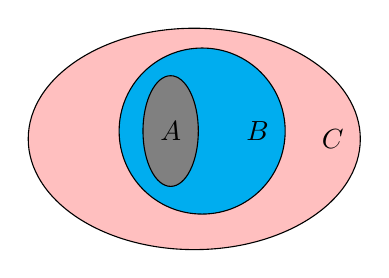
\begin{tikzpicture}
\draw[fill=pink] (0,0) ellipse  (6em and 4em) node [xshift=5em] {$C$};
\draw[fill=cyan] (.1,.1) circle (3em) node [xshift=2em] {$B$};
\draw[fill=gray] (-.3,.1) ellipse (1em and 2em) node {$A$};
\end{tikzpicture}

\tikzsetnextfilename{universal_set}

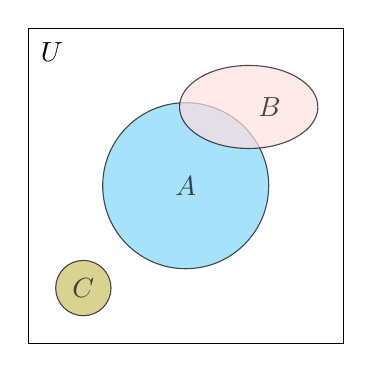
\begin{tikzpicture}
\draw (0,0) -- (4,0) -- (4,4) -- (0,4) -- cycle;
\draw[fill=cyan!50, opacity=.7] (2,2) circle (3em) node {$A$};
\draw[fill=pink!50, opacity=.7] (2.8,3) ellipse  (2.5em and 1.5em) node [right] {$B$};
\draw[fill=olive!50, opacity=.7] (.7,.7) circle  (1em) node {$C$};
\node at (0.3,3.7) {$U$};
\end{tikzpicture}


\tikzsetnextfilename{complement}

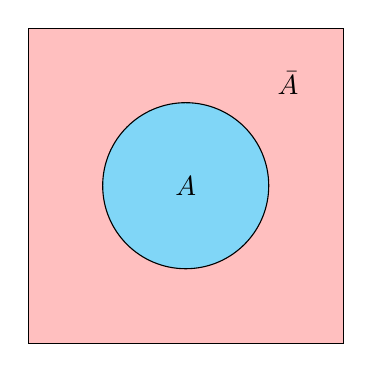
\begin{tikzpicture}
\draw [fill=pink] (0,0) -- (4,0) -- (4,4) -- (0,4) -- cycle;
\draw[fill=cyan!50] (2,2) circle (3em) node {$A$};
\node at (3.3,3.3) {$\bar A$};
\end{tikzpicture}


%%% Some of the following pictures look bad here but they look well in Klatexformula which was used to generate the PNGs

\tikzsetnextfilename{correspondence}

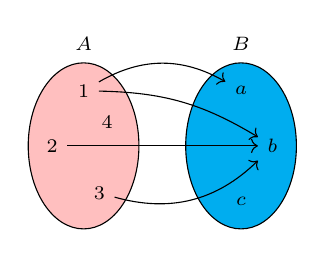
\begin{tikzpicture}
\draw[fill = pink] ellipse (2em and 3em);
\draw[fill = cyan] (2,0) ellipse (2em and 3em);
\node (A) at (0,1.3) {$\scriptstyle A$};
\node (1) at (0,.7) {$\scriptstyle 1$};
\node (4) at (.3,.3) {$\scriptstyle 4$};
\node (2) at (-.4,0) {$\scriptstyle 2$};
\node (3) at (.2,-.6) {$\scriptstyle 3$};
\node (B) at (2,1.3) {$\scriptstyle B$};
\node (a) at (2,.7) {$\scriptstyle a$};
\node (b) at (2.4,0) {$\scriptstyle b$};
\node (c) at (2,-.7) {$\scriptstyle c$};
\draw[->] (1) edge [bend left] (a);
\draw[->] (1) edge [bend left=15] (b);
\draw[->] (2) -- (b);
\draw[->] (3) edge [bend right] (b);
\end{tikzpicture}


\tikzsetnextfilename{map}

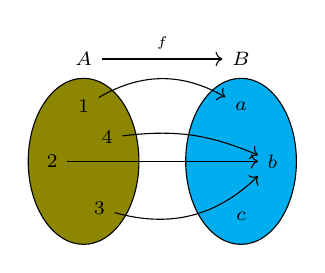
\begin{tikzpicture}
\draw[fill = olive] ellipse (2em and 3em);
\draw[fill = cyan] (2,0) ellipse (2em and 3em);
\node (A) at (0,1.3) {$\scriptstyle A$};
\node (1) at (0,.7) {$\scriptstyle 1$};
\node (4) at (.3,.3) {$\scriptstyle 4$};
\node (2) at (-.4,0) {$\scriptstyle 2$};
\node (3) at (.2,-.6) {$\scriptstyle 3$};
\node (B) at (2,1.3) {$\scriptstyle B$};
\node (a) at (2,.7) {$\scriptstyle a$};
\node (b) at (2.4,0) {$\scriptstyle b$};
\node (c) at (2,-.7) {$\scriptstyle c$};
\draw[->] (A) -- node [above] {$\scriptscriptstyle f$} (B);
\draw[->] (1) edge [bend left] (a);
\draw[->] (4) edge [bend left=15] (b);
\draw[->] (2) -- (b);
\draw[->] (3) edge [bend right] (b);
\end{tikzpicture}

\tikzsetnextfilename{no_map}

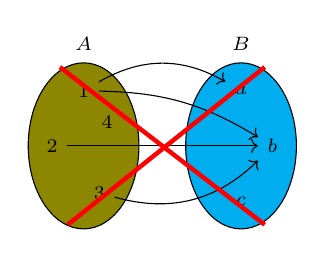
\begin{tikzpicture}
	\draw[fill = olive] ellipse (2em and 3em);
	\draw[fill = cyan] (2,0) ellipse (2em and 3em);
	\node (A) at (0,1.3) {$\scriptstyle A$};
	\node (1) at (0,.7) {$\scriptstyle 1$};
	\node (4) at (.3,.3) {$\scriptstyle 4$};
	\node (2) at (-.4,0) {$\scriptstyle 2$};
	\node (3) at (.2,-.6) {$\scriptstyle 3$};
	\node (B) at (2,1.3) {$\scriptstyle B$};
	\node (a) at (2,.7) {$\scriptstyle a$};
	\node (b) at (2.4,0) {$\scriptstyle b$};
	\node (c) at (2,-.7) {$\scriptstyle c$};
	\draw[->] (1) edge [bend left] (a);
	\draw[->] (1) edge [bend left=15] (b);
	\draw[->] (2) -- (b);
	\draw[->] (3) edge [bend right] (b);
	\draw[-, ultra thick, color = red] (-0.3,1) -- (2.3,-1);
	\draw[-, ultra thick, color = red] (2.3,1) -- (-0.2,-1);
\end{tikzpicture}

\tikzsetnextfilename{noninjective}

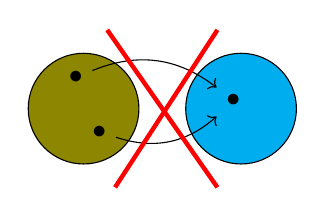
\begin{tikzpicture}
\draw[fill = olive] circle (2em);
\draw[fill = cyan] (2,0) circle (2em);
\node (1) at (-.1,.4) {$\bullet$};
\node (2) at (.2,-.3) {$\bullet$};
\node (a) at (1.9,.1) {$\bullet$};
\draw[->] (1) edge [bend left] (a);
\draw[->] (2) edge [bend right] (a);
\draw[-, ultra thick, color = red] (0.3,1) -- (1.7,-1);
\draw[-, ultra thick, color = red] (1.7,1) -- (0.4,-1);
\end{tikzpicture}



\tikzsetnextfilename{nonsurjective}

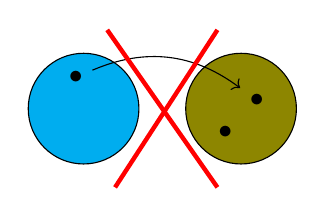
\begin{tikzpicture}
\draw[fill = cyan] circle (2em);
\draw[fill = olive] (2,0) circle (2em);
\node (1) at (-.1,.4) {$\bullet$};
\node (2) at (1.8,-.3) {$\bullet$};
\node (a) at (2.2,.1) {$\bullet$};
\draw[->] (1) edge [bend left] (a);
\draw[-, ultra thick, color = red] (0.3,1) -- (1.7,-1);
\draw[-, ultra thick, color = red] (1.7,1) -- (0.4,-1);
\end{tikzpicture}

\tikzsetnextfilename{direct_image}

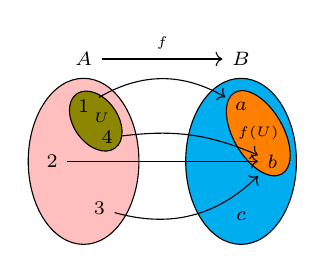
\begin{tikzpicture}
\draw[fill = pink] ellipse (2em and 3em);
\draw[fill = cyan] (2,0) ellipse (2em and 3em);
\draw[fill = olive, rotate=35] (.42,.33) ellipse (.8em and 1.2em);
\draw[fill = orange, rotate=30] (2.1,-.8) ellipse (.9em and 1.7em) node {$\scriptscriptstyle f(U)$};
\node (A) at (0,1.3) {$\scriptstyle A$};
\node at (.23,.55) {$\scriptscriptstyle U$};
\node (1) at (0,.7) {$\scriptstyle 1$};
\node (4) at (.3,.3) {$\scriptstyle 4$};
\node (2) at (-.4,0) {$\scriptstyle 2$};
\node (3) at (.2,-.6) {$\scriptstyle 3$};
\node (B) at (2,1.3) {$\scriptstyle B$};
\node (a) at (2,.7) {$\scriptstyle a$};
\node (b) at (2.4,0) {$\scriptstyle b$};
\node (c) at (2,-.7) {$\scriptstyle c$};
\draw[->] (A) -- node [above] {$\scriptscriptstyle f$} (B);
\draw[->] (1) edge [bend left] (a);
\draw[->] (4) edge [bend left=15] (b);
\draw[->] (2) -- (b);
\draw[->] (3) edge [bend right] (b);
\end{tikzpicture}

\tikzsetnextfilename{inverse_image}

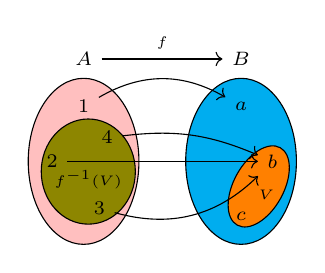
\begin{tikzpicture}
\draw[fill = pink] ellipse (2em and 3em);
\draw[fill = cyan] (2,0) ellipse (2em and 3em);
\draw[fill = olive] (.06,-.13) ellipse (1.7em and 1.9em) node [yshift=-1mm] {$\scriptscriptstyle f^{-1}(V)$};
\draw[fill = orange, rotate=-29] (2.1,.8) ellipse (.9em and 1.6em) node [yshift = -1mm, xshift=1mm] {$\scriptscriptstyle V$};
\node (A) at (0,1.3) {$\scriptstyle A$};
\node (1) at (0,.7) {$\scriptstyle 1$};
\node (4) at (.3,.3) {$\scriptstyle 4$};
\node (2) at (-.4,0) {$\scriptstyle 2$};
\node (3) at (.2,-.6) {$\scriptstyle 3$};
\node (B) at (2,1.3) {$\scriptstyle B$};
\node (a) at (2,.7) {$\scriptstyle a$};
\node (b) at (2.4,0) {$\scriptstyle b$};
\node (c) at (2,-.7) {$\scriptstyle c$};
\draw[->] (A) -- node [above] {$\scriptscriptstyle f$} (B);
\draw[->] (1) edge [bend left] (a);
\draw[->] (4) edge [bend left=15] (b);
\draw[->] (2) -- (b);
\draw[->] (3) edge [bend right] (b);
\end{tikzpicture}


\tikzsetnextfilename{exponential}

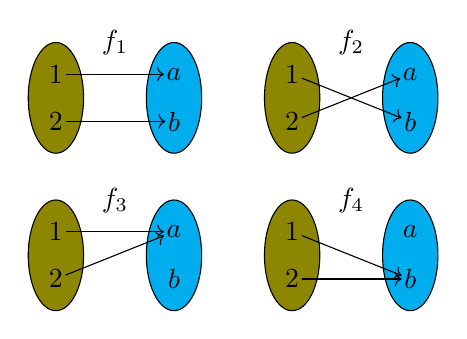
\begin{tikzpicture}[every node/.style={inner sep=1,outer sep=0}]
	\draw[fill = olive] ellipse (1em and 2em);
	\draw[fill = cyan] (1.5,0) ellipse (1em and 2em);
	\node at (.75,.7) {$f_1$};
	\node (1) at (0,.3) {$1$};
	\node (2) at (0,-.3) {$2$};
	\node (a) at (1.5,.3) {$a$};
	\node (b) at (1.5,-.3) {$b$};
	\draw[->] (1) edge (a);
	\draw[->] (2) edge (b);
	\begin{scope}[shift={(3,0)}]
	\draw[fill = olive] ellipse (1em and 2em);
	\draw[fill = cyan] (1.5,0) ellipse (1em and 2em);
	\node at (.75,.7) {$f_2$};
	\node (1) at (0,.3) {$1$};
	\node (2) at (0,-.3) {$2$};
	\node (a) at (1.5,.3) {$a$};
	\node (b) at (1.5,-.3) {$b$};
	\draw[->] (1) edge (b);
	\draw[->] (2) edge (a);
	\end{scope}
	\begin{scope}[shift={(0,-2)}]
	\draw[fill = olive] ellipse (1em and 2em);
	\draw[fill = cyan] (1.5,0) ellipse (1em and 2em);
	\node at (.75,.7) {$f_3$};
	\node (1) at (0,.3) {$1$};
	\node (2) at (0,-.3) {$2$};
	\node (a) at (1.5,.3) {$a$};
	\node (b) at (1.5,-.3) {$b$};
	\draw[->] (1) edge (a);
	\draw[->] (2) edge (a);
	\end{scope}
	\begin{scope}[shift={(3,-2)}]
	\draw[fill = olive] ellipse (1em and 2em);
	\draw[fill = cyan] (1.5,0) ellipse (1em and 2em);
	\node at (.75,.7) {$f_4$};
	\node (1) at (0,.3) {$1$};
	\node (2) at (0,-.3) {$2$};
	\node (a) at (1.5,.3) {$a$};
	\node (b) at (1.5,-.3) {$b$};
	\draw[->] (1) edge (b);
	\draw[->] (2) edge (b);
	\end{scope}
\end{tikzpicture}



\tikzsetnextfilename{partition}

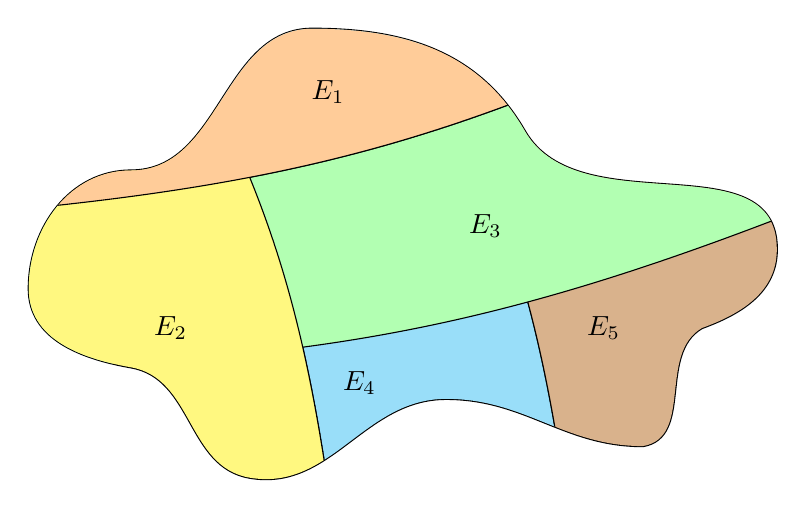
\begin{tikzpicture}
\path
coordinate (aux0) at (0,1.5)
coordinate (aux1) at (0,3.5)
coordinate (aux2) at (10,3.5)
coordinate (aux3) at (9,6)
coordinate (aux4) at (4,0)
coordinate (aux5) at (7,0)
coordinate (aux6) at (2,6)
coordinate (aux7) at (5,6)
coordinate (esp1) at (0.2,2.5)
coordinate (esp2) at (1.5,1.5)
coordinate (esp3) at (3,0.1)
coordinate (esp4) at (5.5,1.1)
coordinate (esp5) at (8,0.5)
coordinate (esp6) at (8.75,2)
coordinate (esp7) at (9.7,3)
coordinate (esp8) at (6.5,4.5)
coordinate (esp9) at (3.8,5.8)
coordinate (esp10) at (1.5,4)
;
\draw[line width=0.8pt]
(esp1) to[out=-90,in=170]
(esp2) to[out=-10,in=170]
(esp3) to[out=-10,in=180]
(esp4) to[out=0,in=180]
(esp5) to[out=10,in=-150]
(esp6) to[out=20,in=-90]
(esp7) to[out=90,in=-60]
(esp8) to[out=120,in=0]
(esp9) to[out=180,in=0]
(esp10) to[out=180,in=90]
cycle;    
\clip
(esp1) to[out=-90,in=170]
(esp2) to[out=-10,in=170]
(esp3) to[out=-10,in=180]
(esp4) to[out=0,in=180]
(esp5) to[out=10,in=-150]
(esp6) to[out=20,in=-90]
(esp7) to[out=90,in=-60]
(esp8) to[out=120,in=0]
(esp9) to[out=180,in=0]
(esp10) to[out=180,in=90]
cycle;    
\filldraw[fill=cyan!40]
(aux4) to[bend right=10]
(aux6) --
(aux7) to[bend left=10]
(aux5) -- cycle;
\filldraw[fill=brown!60]
(aux5) to[bend right=10]
(aux7) --
(10,6) --
(10,0) -- cycle;
\filldraw[fill=green!30]
(aux0) -- 
(aux1) to[bend right=10]
(aux3) --
(10,6) -- 
(aux2) to[bend left=10] cycle;
\filldraw[fill=yellow!50]
(0,0) -- 
(aux4) to[bend right=10]
(aux6) --
(0,6) -- 
(0,0) -- cycle;
\filldraw[fill=orange!40]
(0,6) -- 
(aux1) to[bend right=10]
(aux3) --
(0,6) -- cycle;
\node at (4,5) {$E_1$};  
\node at (2,2) {$E_2$};  
\node at (6,3.3) {$E_3$};  
\node at (4.4,1.3) {$E_4$};  
\node at (7.5,2) {$E_5$};  
\end{tikzpicture}



\tikzsetnextfilename{permutation}

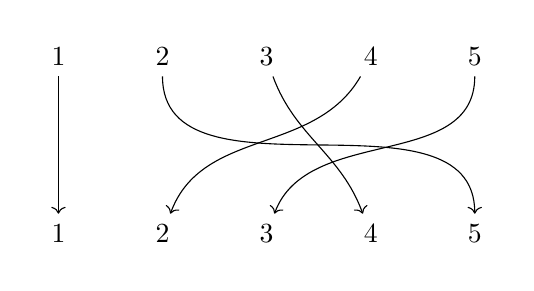
\begin{tikzpicture}[commutative diagrams/every diagram]
\matrix[matrix of math nodes, name=m, commutative diagrams/every cell, row sep = 50] {
	1&2&3&4&5\\
	1&2&3&4&5\\ };
\path[commutative diagrams/.cd, every arrow, every label] (m-1-1) edge (m-2-1);
\path[commutative diagrams/.cd, every arrow, every label] (m-1-2) edge [out=270, in=90] (m-2-5);
\path[commutative diagrams/.cd, every arrow, every label] (m-1-3) edge [out=290, in=110] (m-2-4);
\path[commutative diagrams/.cd, every arrow, every label] (m-1-4) edge [out=240, in=70] (m-2-2);
\path[commutative diagrams/.cd, every arrow, every label] (m-1-5) edge [out=270, in=70] (m-2-3);
\end{tikzpicture}


\tikzsetnextfilename{permutation_sign}

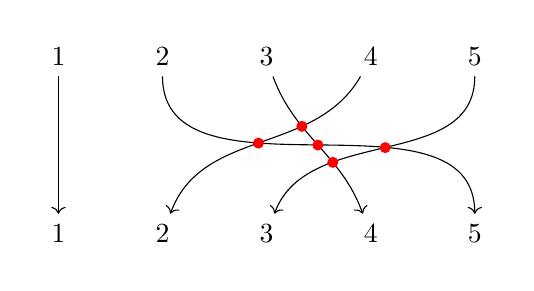
\begin{tikzpicture}[commutative diagrams/every diagram]
\matrix[matrix of math nodes, name=m, commutative diagrams/every cell, row sep = 50] {
	1&2&3&4&5\\
	1&2&3&4&5\\ };
\path[commutative diagrams/.cd, every arrow, every label] (m-1-1) edge (m-2-1);
\path[commutative diagrams/.cd, every arrow, every label] (m-1-2) edge [out=270, in=90, name path= line 2] (m-2-5);
\path[commutative diagrams/.cd, every arrow, every label] (m-1-3) edge [out=290, in=110, name path= line 3] (m-2-4);
\path[commutative diagrams/.cd, every arrow, every label] (m-1-4) edge [out=240, in=70, name path= line 4] (m-2-2);
\path[commutative diagrams/.cd, every arrow, every label] (m-1-5) edge [out=270, in=70, name path= line 5] (m-2-3);
\fill[red,name intersections={of=line 2 and line 3}] (intersection-1) circle (2pt);
\fill[red,name intersections={of=line 2 and line 4}] (intersection-1) circle (2pt);
\fill[red,name intersections={of=line 2 and line 5}] (intersection-1) circle (2pt);
\fill[red,name intersections={of=line 3 and line 4}] (intersection-1) circle (2pt);
\fill[red,name intersections={of=line 3 and line 5}] (intersection-1) circle (2pt);
\end{tikzpicture}

\tikzsetnextfilename{cycle}

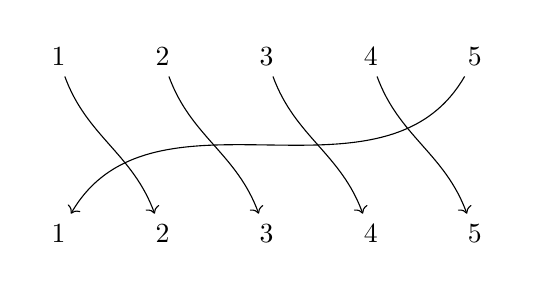
\begin{tikzpicture}[commutative diagrams/every diagram]
\matrix[matrix of math nodes, name=m, commutative diagrams/every cell, row sep = 50] {
1 & 
2 &
3 &
4 &
5 \\
1&2&3&4&5 \\ };
\path[commutative diagrams/.cd, every arrow, every label]
(m-1-1) edge [out=290, in=110] (m-2-2) 
(m-1-2) edge [out=290, in=110] (m-2-3) 
(m-1-3) edge [out=290, in=110] (m-2-4) 
(m-1-4) edge [out=290, in=110] (m-2-5) 
(m-1-5) edge [out=240, in=60] (m-2-1) ;
\end{tikzpicture}

\tikzsetnextfilename{cycle2}

	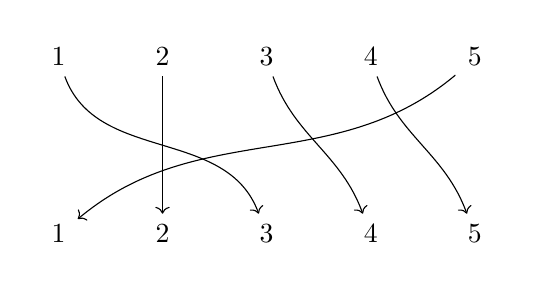
\begin{tikzpicture}[commutative diagrams/every diagram]
	\matrix[matrix of math nodes, name=m, commutative diagrams/every cell, row sep = 50] {
	1 & 
	2 &
	3 &
	4 &
	5 \\
	1&2&3&4&5 \\ };
	\path[commutative diagrams/.cd, every arrow, every label]
	(m-1-1) edge [out=290, in=110] (m-2-3) 
	(m-1-2) edge (m-2-2) 
	(m-1-3) edge [out=290, in=110] (m-2-4) 
	(m-1-4) edge [out=290, in=110] (m-2-5) 
	(m-1-5) edge [out=220, in=40] (m-2-1) ;
	\end{tikzpicture}


\tikzsetnextfilename{cycle3}

	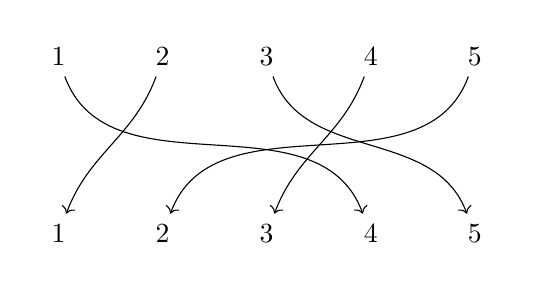
\begin{tikzpicture}[commutative diagrams/every diagram]
	\matrix[matrix of math nodes, name=m, commutative diagrams/every cell, row sep = 50] {
		1&2&3&4&5\\
		1&2&3&4&5\\ };
	\path[commutative diagrams/.cd, every arrow, every label] 
	(m-1-1) edge [out=290, in=110] (m-2-4)
	(m-1-2) edge [out=250, in=70] (m-2-1)
	(m-1-3) edge [out=290, in=110] (m-2-5)
	(m-1-4) edge [out=250, in=70] (m-2-3)
	(m-1-5) edge [out=250, in=70] (m-2-2);
	\end{tikzpicture}

\tikzsetnextfilename{transposition}

	\begin{tikzpicture}[commutative diagrams/every diagram]
	\matrix[matrix of math nodes, name=m, commutative diagrams/every cell, row sep = 50] {
	1 & 
	2 &
	3 &
	4 &
	5 \\
	1&2&3&4&5 \\ };
	\path[commutative diagrams/.cd, every arrow, every label]
	(m-1-1) edge (m-2-1) 
	(m-1-2) edge (m-2-2) 
	(m-1-3) edge [out=290, in=110] (m-2-4) 
	(m-1-4) edge [out=250, in=70] (m-2-3) 
	(m-1-5) edge (m-2-5) ;
	\end{tikzpicture}

\tikzsetnextfilename{transposition2}

	\begin{tikzpicture}[commutative diagrams/every diagram]
	\matrix[matrix of math nodes, name=m, commutative diagrams/every cell, row sep = 50] {
	1 & 
	2 &
	3 &
	4 &
	5 \\
	1&2&3&4&5 \\ };
	\path[commutative diagrams/.cd, every arrow, every label]
	(m-1-1) edge (m-2-1) 
	(m-1-2) edge [out=300, in=90] (m-2-4) 
	(m-1-3) edge (m-2-3) 
	(m-1-4) edge [out=270, in=60] (m-2-2) 
	(m-1-5) edge (m-2-5) ;
	\end{tikzpicture}

\tikzsetnextfilename{circular_cycle}

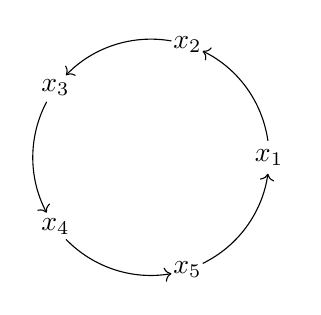
\begin{tikzpicture}
\def \n {5}
\def \radius {1.5cm}
\def \margin {8} % margin in angles, depends on the radius

\foreach \s in {1,...,\n}
{
	\node at ({360/\n * (\s - 1)}:\radius) {$x_{\s}$};
	\draw[->] ({360/\n * (\s - 1)+\margin}:\radius) 
	arc ({360/\n * (\s - 1)+\margin}:{360/\n * (\s)-\margin}:\radius);
}
\end{tikzpicture}

\tikzsetnextfilename{s3}

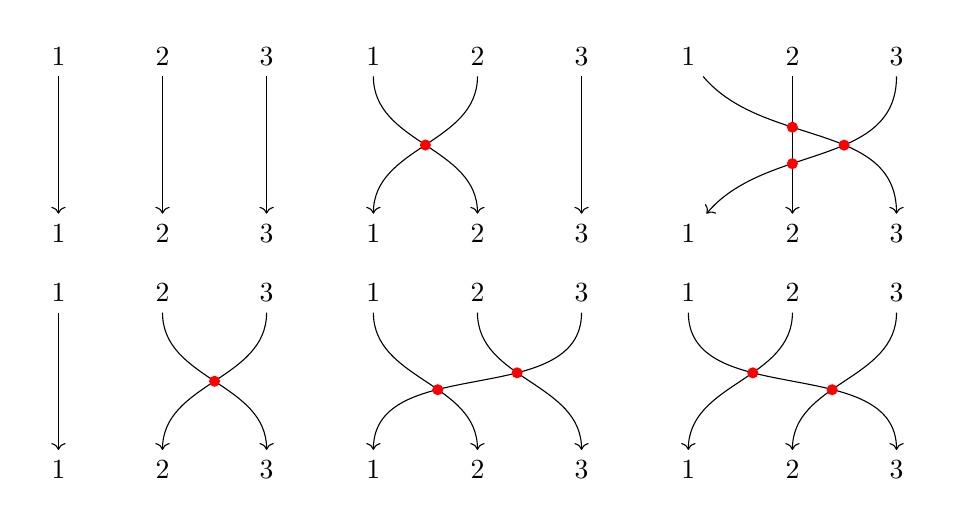
\begin{tikzpicture}[commutative diagrams/every diagram]
	\matrix[matrix of math nodes, name=m, commutative diagrams/every cell, row sep = 50] {
		1&2&3\\
		1&2&3\\ };
	\path[commutative diagrams/.cd, every arrow, every label]
	(m-1-1) edge (m-2-1)
	(m-1-2) edge (m-2-2)
	(m-1-3) edge (m-2-3);
	\begin{scope}[shift={(4,0)}]
	\matrix[matrix of math nodes, name=m, commutative diagrams/every cell, row sep = 50] {
		1&2&3\\
		1&2&3\\ };
	\path[commutative diagrams/.cd, every arrow, every label] 
	(m-1-1) edge [out=270, in=90, name path= line 1] (m-2-2)
	(m-1-2) edge [out=270, in=90, name path= line 2] (m-2-1)
	(m-1-3) edge (m-2-3);
	\fill[red,name intersections={of=line 1 and line 2}] (intersection-1) circle (2pt);
	\end{scope}
	\begin{scope}[shift={(8,0)}]
	\matrix[matrix of math nodes, name=m, commutative diagrams/every cell, row sep = 50] {
		1&2&3\\
		1&2&3\\ };
	\path[commutative diagrams/.cd, every arrow, every label] 
	(m-1-1) edge [out=310, in=90, name path= line 1] (m-2-3)
	(m-1-2) edge [name path= line 2] (m-2-2)
	(m-1-3) edge [out=270, in=50, name path= line 3] (m-2-1);
	\fill[red,name intersections={of=line 1 and line 2}] (intersection-1) circle (2pt);
	\fill[red,name intersections={of=line 1 and line 3}] (intersection-1) circle (2pt);
	\fill[red,name intersections={of=line 2 and line 3}] (intersection-1) circle (2pt);
	\end{scope}
	\begin{scope}[shift={(0,-3)}]
	\matrix[matrix of math nodes, name=m, commutative diagrams/every cell, row sep = 50] {
		1&2&3\\
		1&2&3\\ };
	\path[commutative diagrams/.cd, every arrow, every label] (m-1-1) edge (m-2-1);
	\path[commutative diagrams/.cd, every arrow, every label] (m-1-2) edge [out=270, in=90, name path= line 2] (m-2-3);
	\path[commutative diagrams/.cd, every arrow, every label] (m-1-3) edge [out=270, in=90, name path= line 3] (m-2-2);
	\fill[red,name intersections={of=line 2 and line 3}] (intersection-1) circle (2pt);
	\end{scope}
	\begin{scope}[shift={(4,-3)}]
	\matrix[matrix of math nodes, name=m, commutative diagrams/every cell, row sep = 50] {
		1&2&3\\
		1&2&3\\ };
	\path[commutative diagrams/.cd, every arrow, every label] (m-1-1) edge [out=270, in=90, name path= line 1] (m-2-2);
	\path[commutative diagrams/.cd, every arrow, every label] (m-1-2) edge [out=270, in=90, name path= line 2] (m-2-3);
	\path[commutative diagrams/.cd, every arrow, every label] (m-1-3) edge [out=270, in=90, name path= line 3] (m-2-1);
	\fill[red,name intersections={of=line 1 and line 3}] (intersection-1) circle (2pt);
	\fill[red,name intersections={of=line 2 and line 3}] (intersection-1) circle (2pt);
	\end{scope}
	\begin{scope}[shift={(8,-3)}]
	\matrix[matrix of math nodes, name=m, commutative diagrams/every cell, row sep = 50] {
		1&2&3\\
		1&2&3\\ };
	\path[commutative diagrams/.cd, every arrow, every label] (m-1-1) edge [out=270, in=90, name path= line 1] (m-2-3);
	\path[commutative diagrams/.cd, every arrow, every label] (m-1-2) edge [out=270, in=90, name path= line 2] (m-2-1);
	\path[commutative diagrams/.cd, every arrow, every label] (m-1-3) edge [out=270, in=90, name path= line 3] (m-2-2);
	\fill[red,name intersections={of=line 1 and line 2}] (intersection-1) circle (2pt);
	\fill[red,name intersections={of=line 1 and line 3}] (intersection-1) circle (2pt);
	\end{scope}
\end{tikzpicture}

\tikzsetnextfilename{transsign}

\begin{tikzpicture}[commutative diagrams/every diagram]
\matrix[matrix of math nodes, name=m, commutative diagrams/every cell, row sep = 50] {
	1&\cdots&i&\cdots&j&\dots&n\\
	1&\cdots&i&\cdots&j&\cdots&n\\ };
\path[commutative diagrams/.cd, every arrow, every label] (m-1-1) edge (m-2-1);
\path[commutative diagrams/.cd, every arrow, every label] (m-1-3) edge [out=270, in=90, name path= line 1] (m-2-5);
\path[commutative diagrams/.cd, every arrow, every label] (m-1-5) edge [out=270, in=90, name path= line 2] (m-2-3);
\path[commutative diagrams/.cd, every arrow, every label] (m-1-7) edge (m-2-7);
\path[->] (-1,1.9) edge (-1,.5);
\path[->] (-.75,1.7) edge (-.75,.7);
\path[->] (-.5,1.5) edge (-.5,.9);
\path[->] (1,1.9) edge (1,.5);
\path[->] (.75,1.7) edge (.75,.7);
\path[->] (.5,1.5) edge (.5,.9);
\end{tikzpicture}

\tikzsetnextfilename{forbidden_permutations}

	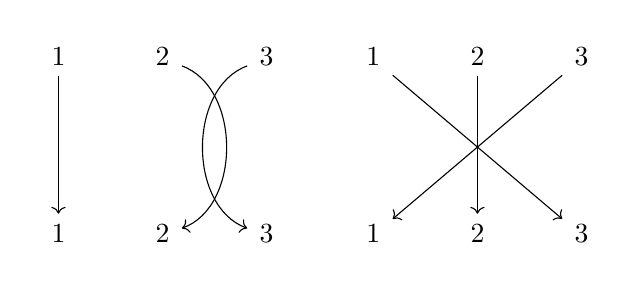
\begin{tikzpicture}[commutative diagrams/every diagram]
	\matrix[matrix of math nodes, name=m, commutative diagrams/every cell, row sep = 50] {
		1&2&3\\
		1&2&3\\ };
	\path[commutative diagrams/.cd, every arrow, every label] (m-1-1) edge (m-2-1);
	\path[commutative diagrams/.cd, every arrow, every label] (m-1-2) edge [bend left = 70] (m-2-2);
	\path[commutative diagrams/.cd, every arrow, every label] (m-1-3) edge [bend right = 70] (m-2-3);
	\begin{scope}[shift={(4,0)}]
	\matrix[matrix of math nodes, name=m, commutative diagrams/every cell, row sep = 50] {
		1&2&3\\
		1&2&3\\ };
	\path[commutative diagrams/.cd, every arrow, every label] (m-1-1) edge (m-2-3);
	\path[commutative diagrams/.cd, every arrow, every label] (m-1-2) edge (m-2-2);
	\path[commutative diagrams/.cd, every arrow, every label] (m-1-3) edge (m-2-1);
	\end{scope}
\end{tikzpicture}

\tikzsetnextfilename{composition}

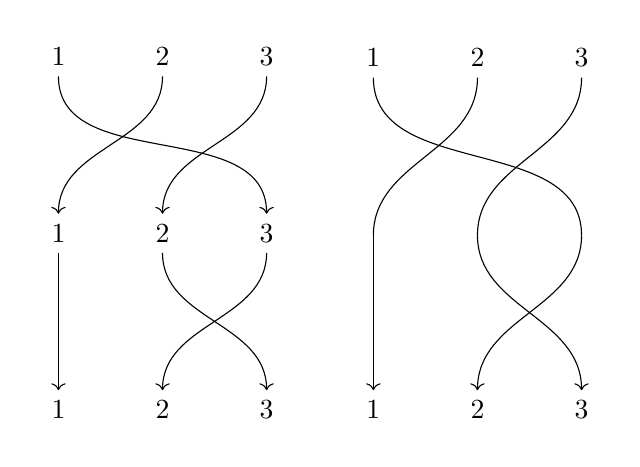
\begin{tikzpicture}[commutative diagrams/every diagram]
\matrix[matrix of math nodes, name=m, commutative diagrams/every cell, row sep = 50] {
	1&2&3\\
	1&2&3\\
	1&2&3\\ };
\path[commutative diagrams/.cd, every arrow, every label] (m-1-1) edge [out=270, in=90] (m-2-3);
\path[commutative diagrams/.cd, every arrow, every label] (m-1-2) edge [out=270, in=90] (m-2-1);
\path[commutative diagrams/.cd, every arrow, every label] (m-1-3) edge [out=270, in=90] (m-2-2);
\path[commutative diagrams/.cd, every arrow, every label] (m-2-1) edge (m-3-1);
\path[commutative diagrams/.cd, every arrow, every label] (m-2-2) edge [out=270, in=90] (m-3-3);
\path[commutative diagrams/.cd, every arrow, every label] (m-2-3) edge [out=270, in=90] (m-3-2);
\begin{scope}[shift={(4,0)}]
\matrix[matrix of math nodes, name=m, commutative diagrams/every cell, row sep = 50] {
	1&2&3\\[6]
	{}&{}&{}\\
	1&2&3\\ };
\path (m-1-1) edge [out=270, in=90] (m-2-3.center)
(m-2-3.center) edge [->, out=270, in=90] (m-3-2);
\path (m-1-2) edge [out=270, in=90] (m-2-1.center)
(m-2-1.center) edge [->] (m-3-1);
\path (m-1-3) edge [out=270, in=90] (m-2-2.center) 
(m-2-2.center) edge [->, out=270, in=90] (m-3-3);
\end{scope}
\end{tikzpicture}

\tikzsetnextfilename{canonica}

	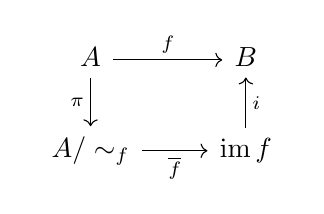
\begin{tikzpicture}[commutative diagrams/every diagram]
	\matrix[matrix of math nodes, name=m, commutative diagrams/every cell] {
	A & 
	B \\
	A/\sim_f &
	\operatorname{im} f \\ };
	\path[commutative diagrams/.cd, every arrow, every label]
	(m-1-1) edge node {$f$} (m-1-2) 
			edge node [swap] {$\pi$} (m-2-1) 
	(m-2-1) edge node [swap] {$\overline{f}$} (m-2-2)
	(m-2-2) edge node [swap] {$i$} (m-1-2);
	\end{tikzpicture}

\tikzsetnextfilename{isomorfiagrupos}

	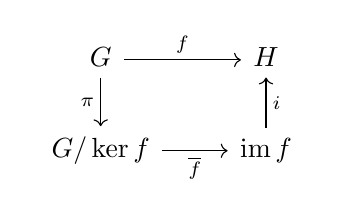
\begin{tikzpicture}[commutative diagrams/every diagram]
	\matrix[matrix of math nodes, name=m, commutative diagrams/every cell] {
	G & 
	H \\
	G/\ker f &
	\operatorname{im} f \\ };
	\path[commutative diagrams/.cd, every arrow, every label]
	(m-1-1) edge node {$f$} (m-1-2) 
			edge node [swap] {$\pi$} (m-2-1) 
	(m-2-1) edge node [swap] {$\overline{f}$} (m-2-2)
	(m-2-2) edge node [swap] {$i$} (m-1-2);
	\end{tikzpicture}

\tikzsetnextfilename{isomorfianillos}

	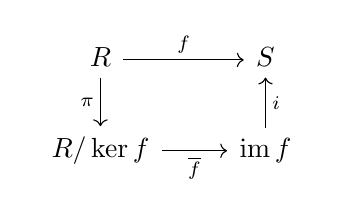
\begin{tikzpicture}[commutative diagrams/every diagram]
	\matrix[matrix of math nodes, name=m, commutative diagrams/every cell] {
	R & 
	S \\
	R/\ker f &
	\operatorname{im} f \\ };
	\path[commutative diagrams/.cd, every arrow, every label]
	(m-1-1) edge node {$f$} (m-1-2) 
			edge node [swap] {$\pi$} (m-2-1) 
	(m-2-1) edge node [swap] {$\overline{f}$} (m-2-2)
	(m-2-2) edge node [swap] {$i$} (m-1-2);
	\end{tikzpicture}

\end{document}